
\documentclass{beamer}
\usepackage{graphicx}
\usepackage[utf8]{inputenc}
\usepackage[T1]{fontenc}
\usepackage[spanish]{babel}

\setbeamerfont{page number in head/foot}{size=\large}
\setbeamertemplate{footline}[frame number]
\setbeamertemplate{navigation symbols}{}%remove navigation symbols

\begin{document}
\graphicspath{ {figs/} }


\title{Probabilistic Numerics}
\author{Federico Zertuche, UTA}
\date{\today}

\frame{\titlepage}

% \frame{\frametitle{Table of contents}\tableofcontents}


\section{Section 1}
\frame{\frametitle{Un problema - de [Henning, Girolami, RSPA 2015]}
\begin{equation*}
  \Large \Large f(x) = e^{\sin^2(3x) - x^2}
\end{equation*}
\par
Problema:
\par
Calcular
\begin{equation*}
  \Large \Large F = \int_0^1 e^{\sin^2(3x) - x^2} dx
\end{equation*}
\begin{figure}[h]

    \includegraphics[scale=0.5]{fx}
    % \caption{}
\end{figure}
}


\frame{ \frametitle{Un problema - de estimación}
\begin{itemize}
  \item No tengo una fórmula para $F$.
  \item Puedo evaluar $f(x)$.
\end{itemize}
\par
Estimar:
\begin{equation*}
  \Large \Large F = \int_0^1 e^{\sin^2(3x) - x^2} dx
\end{equation*}
Usando:
\begin{equation*}
  f(x_1), f(x_2), ... , f(x_n)
\end{equation*}
}

\frame{ \frametitle{Un problema -  de muetras aleatorias?}
\begin{equation*}
  \tilde{F} \propto \dfrac{1}{N} \sum_{i=1}^N f(x) \ (casi)
  % \dfrac{Z}{N} \sum_{i=1}^N \dfrac{f(x)}{g(x)} \dfrac{g(x)}{Z}
\end{equation*}
\begin{figure}[h]
  \centering
    \begin{subfigure}{}
      \centering
        \includegraphics[width=.48\linewidth]{UnifF}
    \end{subfigure}
    \begin{subfigure}{}
        \centering
        \includegraphics[width=.48\linewidth]{GaussF}
    \end{subfigure}%
    \label{fig:ransSampling}
\end{figure}
}

\frame{ \frametitle{Un problema - de estructura}
En realidad:
\begin{enumerate}
  \item Puedo evaluar $f(x)$. %\pause
  \item Se que $f$ es continua. %\pause
\end{enumerate}
\par
Voy a asumir:
\begin{equation*}
  f \sim \mathcal{GP}\left(m(x), \ k(x,x')\right) .
\end{equation*}
Como $\int$ es lineal:
\begin{equation*}
  F  = \int f \sim \mathcal{N}\left(m_{\int}, \ k_{\int \int}\right)
\end{equation*}
donde
\begin{align*}
  m_{\int}(x) &= \int m dx \\
  k_{\int \int} &= \int \int k dx dx' .
\end{align*}
}

\frame{\frametitle{Un problema - de estructura}
Tengo una descripción formal de como es - mas o menos - $F$.
La incertidumbre que tengo sobre $f$ se propaga a su integral:
\par
\vspace{1em}
Sería cool tener la distribución de $F|f(x)$.
\begin{equation*}
  \Large  F \mid f(x)  \sim \mathcal{N}\left(\ m_{F \mid f(x)}\left(x, f(x)\right),\ k_{F \mid f(x)}(x) \ \right)
\end{equation*}
donde
\begin{align*}
  \Large m_{F \mid f(x)}\left(x, f(x)\right) &:= k_{\int}(x) k(x,x)^{-1} f(x) \\
  \Large k_{F \mid f(x)}(x) &:= k_{\int \int} - k_{\int}(x) k(x,x)^{-1} k_{\int}(x)
\end{align*}
}


\frame{\frametitle{Un problema - de uso}
Cuál es mi estiamción de $F$?\\
Qué tal $m_{F \mid f(x)}\left(x, f(x)\right)$?
\par
\vspace{2em}
Dónde les gustaría evlauar $f$? \\
Qué tal en el lugar donde $k_{F \mid f(x)}(x)$ es grande?

}

\frame{\frametitle{Un problema - de uso}
Un modelo para $f$:

\begin{figure}[h]
    \centering
    \begin{subfigure}{}
        \centering
        \includegraphics[width=.48\linewidth]{LSKern}
    \end{subfigure}
    \begin{subfigure}{}
        \centering
        \includegraphics[width=.48\linewidth]{samples}
    \end{subfigure}%
    \label{fig:lskernel}
\end{figure}
}

\frame{\frametitle{Un problema - de uso}
Una evaluación de $f$:

\Large
\begin{equation*}
      \begin{aligned}
      & \underset{x}{\text{maximize}}
      & & k_{F \mid f(x)}(x) \\
      \end{aligned}
\end{equation*}

\begin{figure}[h]
    \centering
    \begin{subfigure}{}
        \centering
        \includegraphics[width=.48\linewidth]{PosteriorVariance1d}
    \end{subfigure}
    \begin{subfigure}{}
        \centering
        \includegraphics[width=.48\linewidth]{PosteriorSamples1}
    \end{subfigure}%
    \label{fig:firsteval}
\end{figure}
}

\frame{\frametitle{Un problema - de uso}
Dos evaluaciones de $f$:
\Large
\begin{equation*}
      \begin{aligned}
      & \underset{x}{\text{maximize}}
      & & k_{F \mid f(x_1), f(x_2)}(x_1, x_2) \\
      \end{aligned}
\end{equation*}

\begin{figure}[h]
    \centering
    \begin{subfigure}{}
        \centering
        \includegraphics[width=.48\linewidth]{PosteriorVariance2d}
    \end{subfigure}
    \begin{subfigure}{}
        \centering
        \includegraphics[width=.48\linewidth]{PosteriorSamples2}
    \end{subfigure}%
    \label{fig:secondteval}
\end{figure}

}

\frame{\frametitle{Un problema - de trapazides}
Qué tengo al final? El método del trapezoide!
\begin{figure}[h]
    \includegraphics[scale=0.5]{postMean}
    % \caption{}
\end{figure}
}


\frame{\frametitle{Proba Numerics}
Modela incertidumbre numérica que se propaga.
\begin{enumerate}
  \item Produce medidas de proba sobre todas las incógnitas.
  \item La etructura en los errores puede ser propagada a otras operaciones posteriores.
  \item Usar stats para determinar puntos inportantes (alocación de recursos).
  \item Nueva perspectiva para diseñar algos.
\end{enumerate}

}

\frame{ \frametitle{Proba Numerics - Fluidos}
Simular un fluido:
\begin{enumerate}
  \item Escoger una equation. %\pause
  \item Escoger el valor de algunos parámetros. %\pause
  \item Decidir cuál método numérico usar. %\pause
  \item Calcular la sol numérica %\pause
\end{enumerate}
\par
Qué tan seguros de la solución estamos? (No mucho) %\pause
}


\frame{\frametitle{Proba Numerics - Fluidos[Chkrebtii, Bayesian Analysis 2016]}
\begin{figure}[h]

    \includegraphics[scale=0.7]{vorticity}
    % \caption{}
\end{figure}
}


\frame{\frametitle{Probabilidades}
Marco cuantitativo para la inferencia científica.
\vspace{2em}
\begin{itemize}
\item[] Describe incertidumbre en experimentos
\item[] PERO TAMBIEN
\item[] sirve para cuantificar incertidumbre \emph{epistémica}.
\end{itemize}
}

\frame{\frametitle{Gracias!}
\begin{figure}[h]
    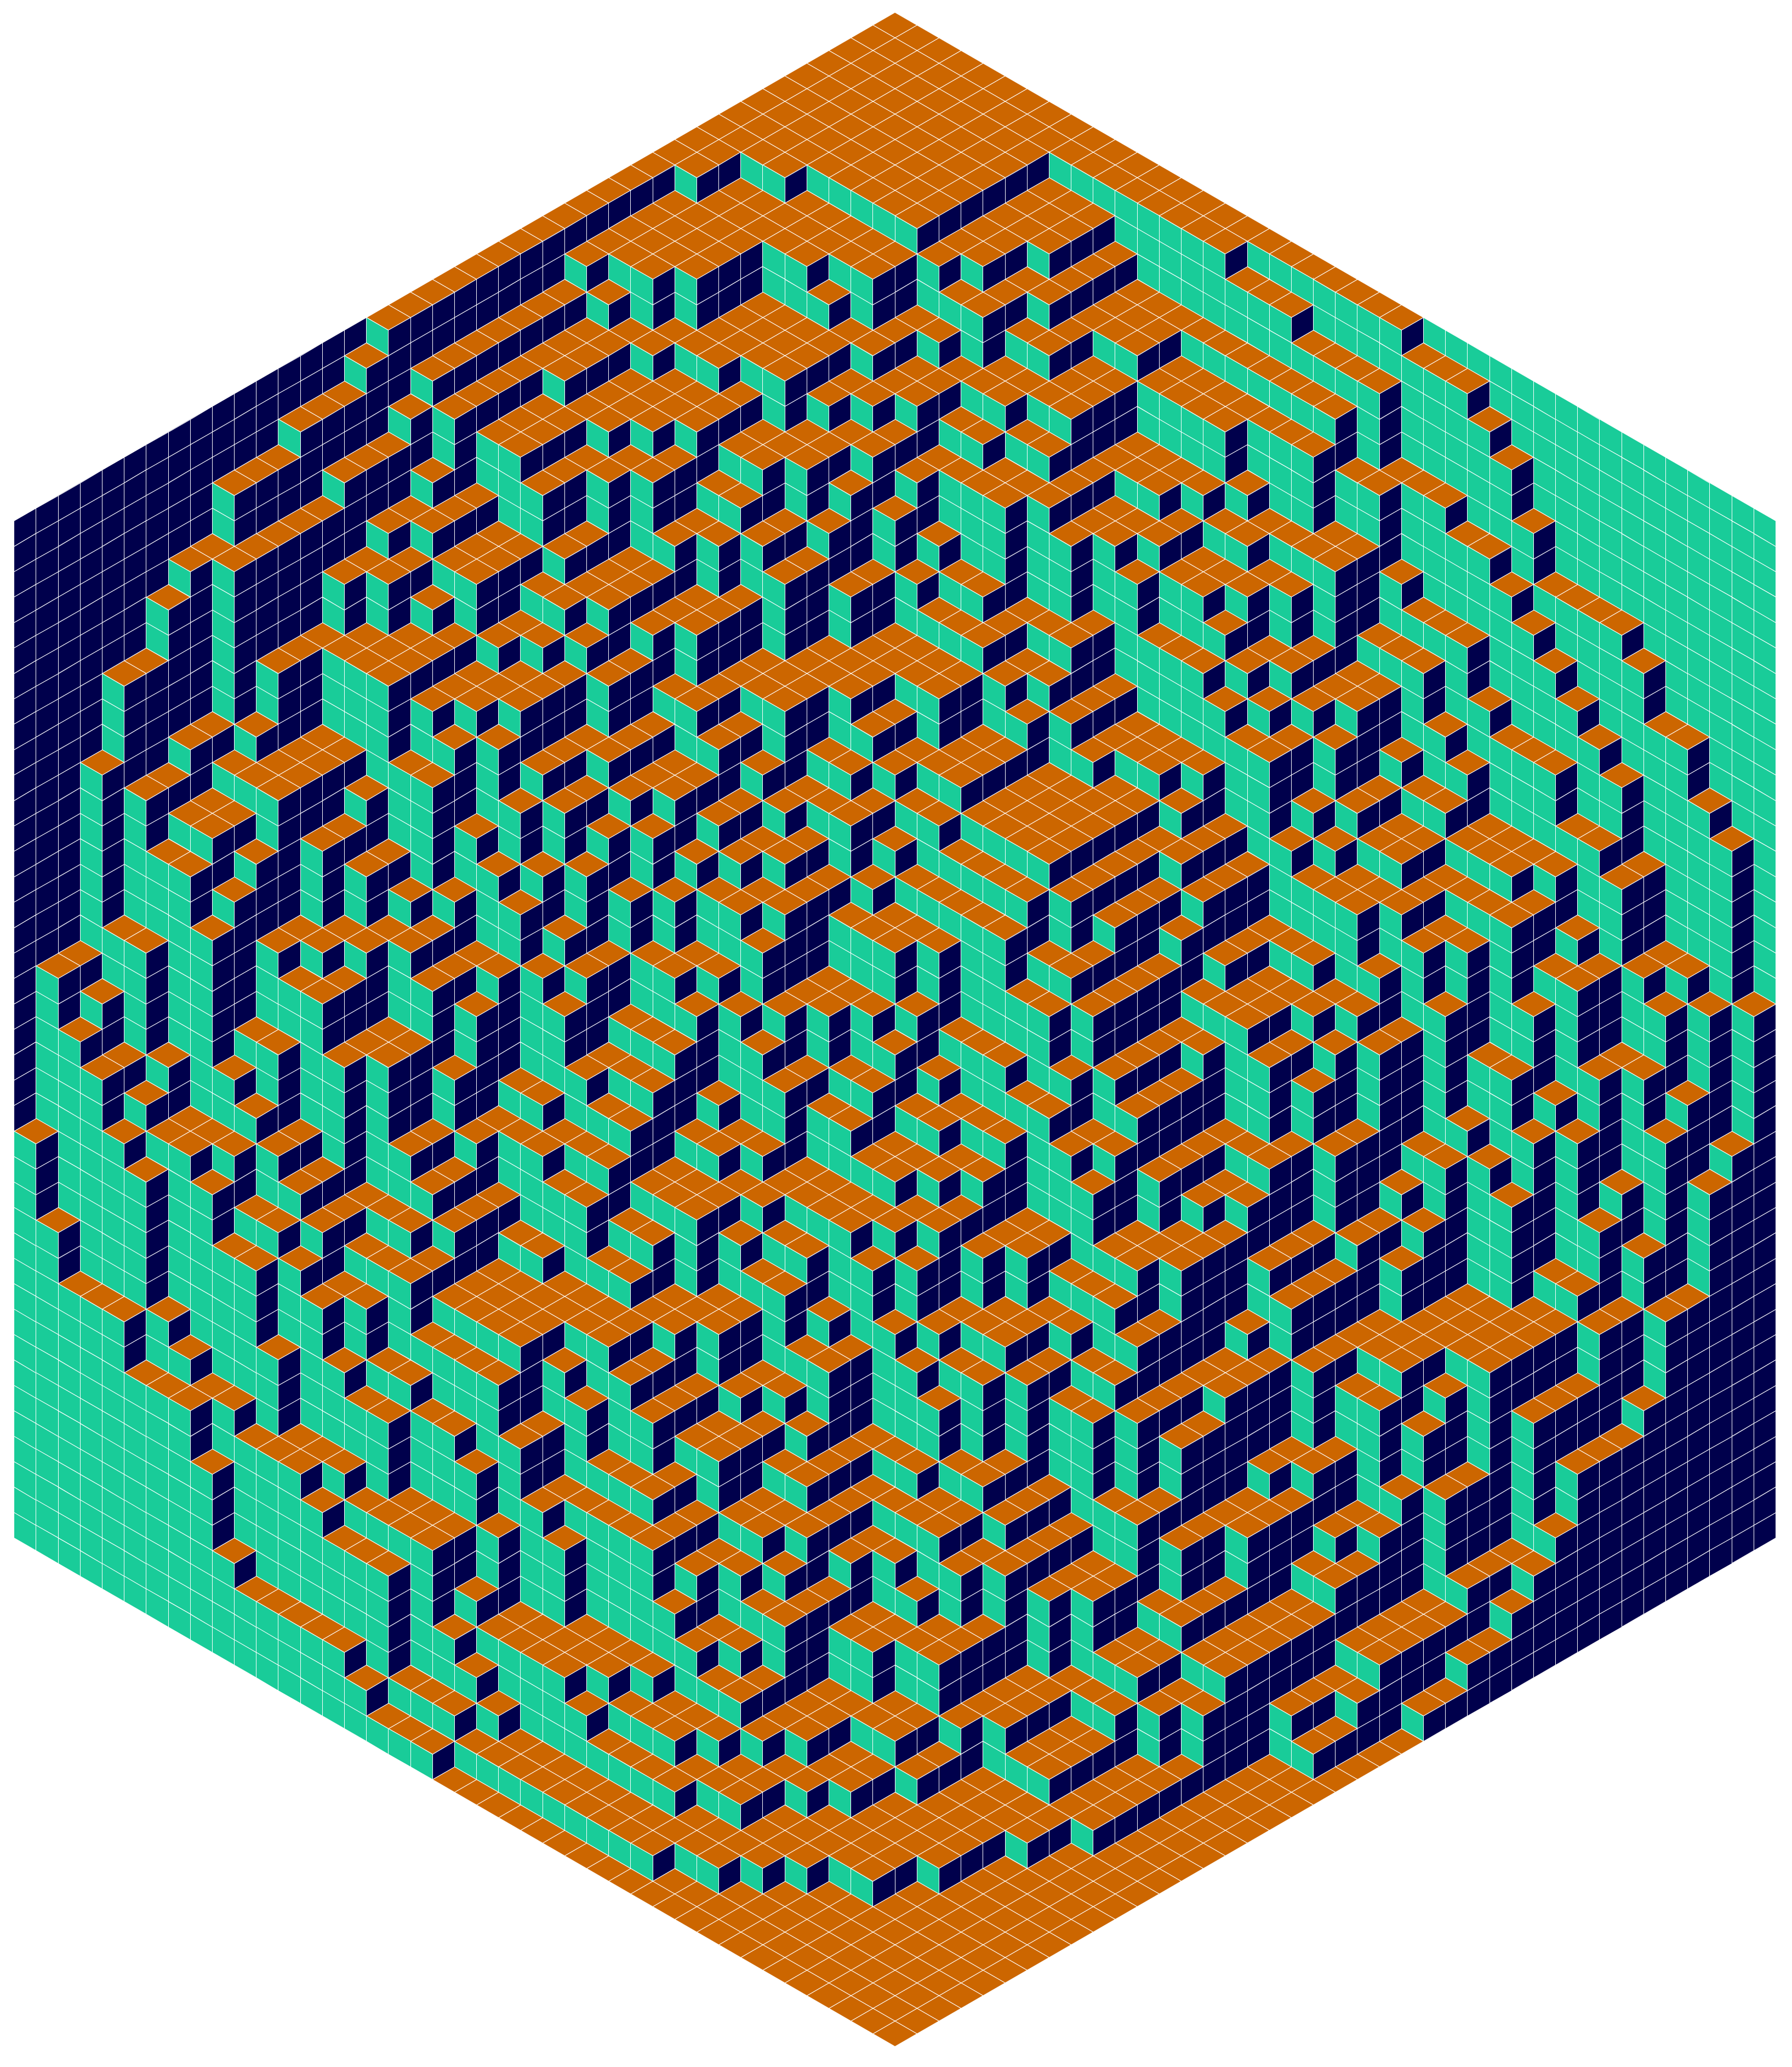
\includegraphics[scale=0.75]{hex}
    % \caption{}
\end{figure}
}

\end{document}
